% 《物理实验报告模板.tex》的共同版式；所有实验模板均载入本文件。
\documentclass[UTF8,a4paper,10pt,fontset=fandol]{ctexart}
\usepackage[left=3.175cm,right=3.175cm,top=2.54cm,bottom=2.54cm]{geometry}
\usepackage{graphicx,tikz,pgfplots,needspace,adjustbox,booktabs,fancyhdr,lastpage,amsmath,amssymb,array,tabularx,longtable}
\pgfplotsset{compat=1.18}
\setlength{\parindent}{0pt}
\setlength{\parskip}{2pt}
\setlength{\headheight}{18pt}
\linespread{1}
\newcommand{\SetField}[2]{\expandafter\def\csname reportfield@#1\endcsname{#2}}
\makeatletter
\newcommand{\Field}[2][1.35cm]{%
  \ifcsname reportfield@#2\endcsname
    \expandafter\ifx\csname reportfield@#2\endcsname\@empty
      \underline{\makebox[#1]{\strut}}%
    \else\csname reportfield@#2\endcsname\fi
  \else\underline{\makebox[#1]{\strut}}\fi}
\makeatother
\newcommand{\MathField}[2][1.35cm]{%
  \ifcsname reportfield@math_#2\endcsname
    \csname reportfield@math_#2\endcsname
  \else\text{\Field[#1]{#2}}\fi}
\newcommand{\coverfield}[2]{%
  \noindent{\heiti\fontsize{18pt}{48pt}\selectfont
  \makebox[3.3cm][l]{#1}\underline{\makebox[8.8cm][c]{\Field[0pt]{#2}}}\par}}
\newcommand{\bindingline}[1][2.85]{%
  \begin{tikzpicture}[remember picture,overlay]
    \foreach \i in {0,...,38}{%
      \pgfmathsetmacro{\bindingy}{-#1-0.52*\i}%
      \ifnum\i=13\relax
        \node[inner sep=0pt] at ([xshift=1.05cm,yshift=\bindingy cm]current page.north west) {\songti\fontsize{10.5pt}{10.5pt}\selectfont 装};
      \else\ifnum\i=19\relax
        \node[inner sep=0pt] at ([xshift=1.05cm,yshift=\bindingy cm]current page.north west) {\songti\fontsize{10.5pt}{10.5pt}\selectfont 订};
      \else\ifnum\i=25\relax
        \node[inner sep=0pt] at ([xshift=1.05cm,yshift=\bindingy cm]current page.north west) {\songti\fontsize{10.5pt}{10.5pt}\selectfont 线};
      \else
        \pgfmathsetmacro{\bindingtop}{\bindingy+0.20}%
        \pgfmathsetmacro{\bindingbottom}{\bindingy-0.20}%
        \draw[line width=0.35pt,dash pattern=on 1.2pt off 1.8pt]
          ([xshift=1.05cm,yshift=\bindingtop cm]current page.north west)
          -- ([xshift=1.05cm,yshift=\bindingbottom cm]current page.north west);
      \fi\fi\fi}
  \end{tikzpicture}%
}
% 装订线印在每一页正文和原始数据页，续页也沿用母模板样式。
\newif\ifreportbinding
\AddToHook{shipout/foreground}{\ifreportbinding\bindingline\fi}
\fancypagestyle{report}{\fancyhf{}\fancyfoot[C]{第\thepage 页\quad 共\pageref{LastPage}页}\renewcommand{\headrulewidth}{0.4pt}}
\fancypagestyle{record}{\fancyhf{}\fancyhead[C]{原始数据记录单}\fancyfoot[C]{第\thepage 页\quad 共\pageref{LastPage}页}\renewcommand{\headrulewidth}{0.4pt}}
\newcommand{\ReportCover}[1]{%
  \thispagestyle{empty}\vspace*{1.0cm}
  \begin{center}
    
\includegraphics[width=8.184cm]{tongji_logo.jpeg}\par
    {\bfseries\fontsize{18pt}{24pt}\selectfont TONGJI UNIVERSITY\par}
    \vspace{1.5cm}{\heiti\fontsize{36pt}{44pt}\selectfont 物理实验报告\par}
  \end{center}
  \vspace{1.5cm}
  \coverfield{实验名称}{experiment}
  \coverfield{学生姓名}{student}
  \coverfield{学\hspace{1em}号}{student_id}
  \coverfield{组\hspace{1em}号}{group}
  \coverfield{实验日期}{date}
  \clearpage\reportbindingtrue\pagestyle{report}
  \begin{center}{\heiti\fontsize{14pt}{40pt}\selectfont #1\par}\end{center}}
\newcommand{\ReportSection}[1]{\Needspace{4\baselineskip}\par\vspace{0.35\baselineskip}{\heiti #1}\par}
\newcommand{\ReportSubsection}[1]{\Needspace{3\baselineskip}\par\vspace{0.2\baselineskip}{\bfseries #1}\par}
\newif\ifreportimages
\newcommand{\ReportRecord}{%
  \clearpage\thispagestyle{record}
  \vspace*{0.6cm}%
  \ifreportimages\else（请将教师签字的实验数据记录单完整拍照粘贴至此处。）\fi
}

\xeCJKDeclareCharClass{CJK}{"2460 -> "2461}
% ===== 数据输入区开始 =====
\SetField{experiment}{空气比热容比的测定}
% 后端以 \SetField{字段名}{值} 填入数据；缺省值保持空白。
% 母模板封面字段：\Field{experiment} \Field{student} \Field{student_id} \Field{group} \Field{date}
% ===== 数据输入区结束 =====
\begin{document}\fontsize{10.5pt}{20pt}\selectfont
\ReportCover{空气比热容比的测定}
\ReportSection{实验目的}
1. 理解气体的定压、定容比热容及比热容比的物理意义，并认识绝热过程的近似条件。\par
2. 使用振动法测定空气比热容比，掌握小球直径、质量、周期、气压和容积的测量。\par
3. 学习零点修正、重复测量及 A、B 类不确定度的合成，分析直径误差的放大效应。\par
\ReportSection{实验原理}
图4.2.1为振动法测比热容比的实验原理示意图。实验以球形储气瓶中的空气作为研究的热力学系统，并测量其比热容比数值。储气瓶正上方连接一个精密细玻璃管B，其内有一个可以自由移动的振动小球A，侧壁有一个小孔。振动小球A的直径仅比玻璃管B的直径小0.01 mm～0.02 mm。在储气瓶壁上有一小口并插入一根细管C，可将待测气体通过细管C注入到储气瓶中。为了补偿由于空气阻尼以及少量漏气引起的小球A振幅的衰减，可以通过细管C持续稳定注入小气压的气流。如果注入气体的流量适当时，小球A就能在玻璃管B的小孔上下做简谐振动。当振动小球A处于小孔下方的半个振动周期时，注入气体会使储气瓶内的压力增大，引起小球A向上移动。而当小球A处于小孔上方的半个振动周期时，储气瓶内的气体将通过小孔流出，使物体下落，以后重复上述过程。小球A的振动周期$T$可利用光电计时装置来测得。
\begin{center}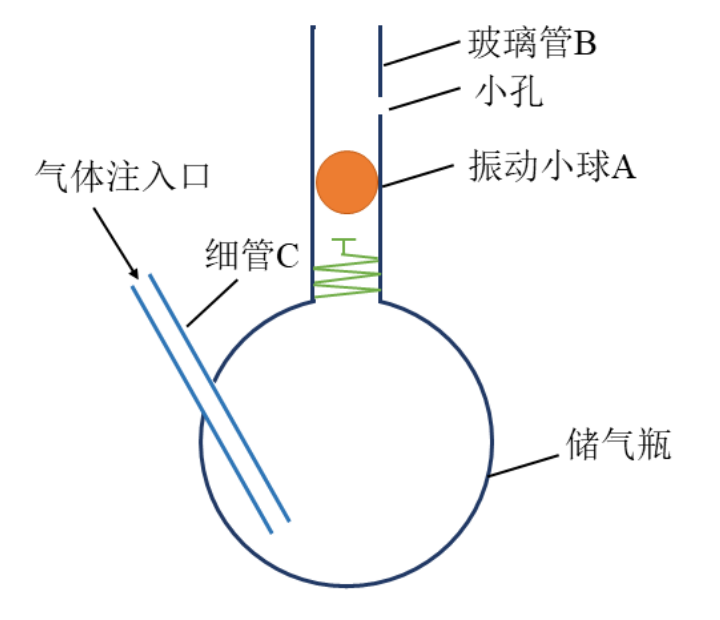
\includegraphics[width=5.4cm]{figures/heat-principle-source.png}\par
{\small 图4.2.1实验原理示意图。}\end{center}
若小球A的质量为$m$，半径为$r$（直径为$d$），当储气瓶内压强$P$满足下面条件时，小球A处于受力平衡状态。
\begin{equation}P=P_L+\frac{mg}{\pi r^2}\tag{4.2.1}\end{equation}
(4.2.1)式中$P_L$为大气压强。

当振动小球A偏离平衡位置一个较小距离$x$时，储气瓶内的压强将变化$dP$。由牛顿第二定律可得物体的运动方程为：
\begin{equation}m\frac{\mathrm d^2x}{\mathrm dt^2}=\pi r^2\mathrm dP\tag{4.2.2}\end{equation}
\Needspace{5\baselineskip}
由于小球振动过程相当快，可以近似作为绝热过程处理，所以球形储气瓶内的气体压强$P$以及气体体积$V$满足绝热方程
\begin{equation}PV^\gamma=C\quad\text{（常数）}\tag{4.2.3}\end{equation}
将(4.2.3)式求导得出$\mathrm dP=-\frac{P\gamma\mathrm dV}{V}$，而玻璃管B内气体的微小增量为
\begin{equation}\mathrm dV=\pi r^2x\tag{4.2.4}\end{equation}
将(4.2.4)式与(4.2.3)式代入(4.2.2)式得
\begin{equation}\frac{\mathrm d^2x}{\mathrm dt^2}+\frac{\pi^2r^4P\gamma}{mV}x=0\tag{4.2.5}\end{equation}
(4.2.5)式即为熟知的简谐振动方程，振动角频率$\omega$为
\begin{equation}\omega=\sqrt{\frac{\pi^2r^4P\gamma}{mV}}=\frac{2\pi}{T}\tag{4.2.6}\end{equation}
化简后可得
\begin{equation}\gamma=\frac{4mV}{T^2Pr^4}=\frac{64mV}{T^2Pd^4}\tag{4.2.7}\end{equation}
若实验直接测得小球的振动周期$T$、小球质量$m$，直径$d$，以及储气瓶体积$V$，并根据(4.2.1)式得到储气瓶内气体压强$P$，那么利用(4.2.7)式即可计算出空气的比热容比$\gamma$值。众所周知，空气是多种气体组成的混合物，其中99\%以上是双原子气体氮和氧，因此经典理论得出空气的$\gamma$值约为1.402。
\ReportSection{实验内容与步骤}
\ReportSubsection{5.1 实验仪器的调整与电路连接}
1.将微型气泵和缓冲瓶用橡皮管连接好，把装有小钢球的细玻璃管插入球形储气瓶中。将光电门利用方形连接块固定在铁架台立杆上，并调节其位置于细玻璃管的小孔附近。\par
2.调节铁架台底板上的三个水平调节螺钉，使底板处于水平状态。\par
3.接通微型气泵电源，微调气泵上的调节旋钮，待球形储气瓶内注入一定压力的气体后，细玻璃管中的钢球将离开弹簧向上方移动，此时应调节好气体流量，使钢球在玻璃管中以小孔为中心做简谐振动。\par
4.将网络型气体比热容比测试仪的电路控制箱与计算机主机以及光电门相连，确认连接无误后，接通电路控制箱的电源。
\ReportSubsection{5.2 小球直径、质量以及大气压强的测量}
1.用螺旋测微计测量备用小球直径$d$，重复测量5次，注意不可取出玻璃管内的小球，以免损坏仪器。\par
2.用空盒气压计在实验开始前和结束时各测一次大气压强$P_L$，并取平均值。\par
3.用物理天平测量备用小球的质量$m$。
\ReportSubsection{5.2 数据上传及周期的测量}
1.接通网络型气体比热容比测试仪并选择实验项目为“①空气”，按“确定”键进入当前实验选项的“参数设置”界面。\par
2.设定测量数据，包括小球直径（5个测量值）、小球质量、储气瓶容积、实验开始时测得的大气压强值。\par
3.通过“测量计数”界面完成小球振动周期的测量，设置振动次数为100次，启动实验装置，完成5次周期值的测量\par
4.再次设定大气压强值，完成实验。\par
5.实验完成后，断开电源，将各部分实验仪器整理好，根据测得的实验数据计算空气的比热容比$\gamma$，估算不确定度，并与理论值比较，计算百分差。
\ReportSection{实验仪器}
网络型气体比热容比测试仪、带小孔细玻璃管和储气瓶、螺旋测微计、电子天平、空盒气压计及计时器。记录各仪器最小分度与估计误差。
\ReportSection{数据记录和处理}
\noindent\Field[0pt]{heat_reading_note}\par
\ReportSubsection{1．小球直径测量（螺旋测微计）：}
\begin{center}{\small 表4.2.2 小球直径测量数据记录表\qquad 单位：mm}\par
\small\renewcommand{\arraystretch}{1.35}
\begin{adjustbox}{max width=\textwidth}
\begin{tabular}{|c|c|c|c|c|c|c|}\hline
测量序号 & 1 & 2 & 3 & 4 & 5 & 平均值\\\hline
初读数 & \Field[8mm]{diameter_initial_01} & \Field[8mm]{diameter_initial_02} & \Field[8mm]{diameter_initial_03} & \Field[8mm]{diameter_initial_04} & \Field[8mm]{diameter_initial_05} & ---\\\hline
末读数 & \Field[8mm]{diameter_final_01} & \Field[8mm]{diameter_final_02} & \Field[8mm]{diameter_final_03} & \Field[8mm]{diameter_final_04} & \Field[8mm]{diameter_final_05} & ---\\\hline
直径 $d$ & \Field[8mm]{diameter_corrected_01} & \Field[8mm]{diameter_corrected_02} & \Field[8mm]{diameter_corrected_03} & \Field[8mm]{diameter_corrected_04} & \Field[8mm]{diameter_corrected_05} & \Field{diameter_mean_mm}\\\hline
\end{tabular}\end{adjustbox}\end{center}
\[U_{dA}=\sqrt{\frac{\sum(d_i-\bar d)^2}{n(n-1)}}=\MathField{diameter_u_a_mm}\,\mathrm{mm}\]
\[U_{dB}=\frac{\MathField{diameter_error_mm}}{\sqrt3}=\MathField{diameter_u_b_mm}\,\mathrm{mm}\]
\[U_d=\sqrt{U_{dA}^2+U_{dB}^2}=\MathField{diameter_mean_u_mm}\,\mathrm{mm},\quad
U_{rd}=\frac{U_d}{\bar d}\times100\%=\MathField{diameter_relative_u_percent}\%\]
\[d=(\MathField{diameter_mean_mm}\pm\MathField{diameter_mean_u_mm})\,\mathrm{mm}\]
\ReportSubsection{2. 小球质量：}
$m=\Field{mass_g}\,\mathrm g$\par
仪器误差$\Delta=\Field{mass_error_g}\,\mathrm g$
\[U_m=\frac{\Delta}{\sqrt3}=\MathField{mass_u_g}\,\mathrm g,\quad
U_{rm}=\frac{U_m}{m}\times100\%=\MathField{mass_relative_u_percent}\%\]
\[m=(\MathField{mass_result_g}\pm\MathField{mass_u_g})\,\mathrm g\]
\ReportSubsection{3. 玻璃容器的体积：}
\[V=\MathField{volume_l}\times10^{-3}\,\mathrm{m^3},\qquad U_V=\MathField{volume_standard_u_l}\times10^{-3}\,\mathrm{m^3}\]
\[U_{rV}=\frac{U_V}{V}\times100\%=\MathField{volume_relative_u_percent}\%\]
\[V=(\MathField{volume_result_m3}\pm\MathField{volume_u_m3})\,\mathrm{m^3}\]
\ReportSubsection{4. 容器中空气压强的测量：}
①大气压强$P_L$：\par
实验开始时：$P_{L1}=\Field{pressure_start_kpa}\,\mathrm{kPa}$\quad
实验结束时：$P_{L2}=\Field{pressure_end_kpa}\,\mathrm{kPa}$\par
平均值$\bar P_L=\MathField{pressure_mean_kpa}\,\mathrm{kPa}$。\par
仪器误差$\Delta=\Field{pressure_error_kpa}\,\mathrm{kPa}$
\[U_{P_L}=\frac{\Delta}{\sqrt3}=\MathField{pressure_mean_u_kpa}\,\mathrm{kPa}\]
\[U_{rP_L}=\frac{U_{P_L}}{P_L}\times100\%=\MathField{pressure_atmos_relative_u_percent}\%\]
\[P_L=(\MathField{pressure_mean_kpa}\pm\MathField{pressure_mean_u_kpa})\,\mathrm{kPa}\]
②容器内的大气压$P$：
\[P=P_L+\frac{4mg}{\pi d^2}=\MathField{pressure_inside_pa}\,\mathrm{Pa}\]
\[U_P\approx U_{P_L}=\MathField{pressure_inside_u_pa}\,\mathrm{Pa},\quad
U_{rP}=\frac{U_P}{P}\times100\%=\MathField{pressure_relative_u_percent}\%\]
\[P=(\MathField{pressure_inside_result_pa}\pm\MathField{pressure_inside_u_pa})\,\mathrm{Pa}\]
\ReportSubsection{5. 小球振动周期$T$的测量：}
\begin{center}{\small 表4.2.3 小球振动周期数据记录表}\par
\small\renewcommand{\arraystretch}{1.35}
\begin{adjustbox}{max width=\textwidth}
\begin{tabular}{|c|c|c|c|c|c|c|}\hline
测量序号 & 1 & 2 & 3 & 4 & 5 & 平均值\\\hline
$100T$（s） & \Field[8mm]{time_100_01} & \Field[8mm]{time_100_02} & \Field[8mm]{time_100_03} & \Field[8mm]{time_100_04} & \Field[8mm]{time_100_05} & \Field{period_time_mean_s}\\\hline
$T$（s） & \Field[8mm]{period_calculated_01} & \Field[8mm]{period_calculated_02} & \Field[8mm]{period_calculated_03} & \Field[8mm]{period_calculated_04} & \Field[8mm]{period_calculated_05} & \Field{period_mean_s}\\\hline
\end{tabular}\end{adjustbox}\end{center}
\[U_{TA}=\sqrt{\frac{\sum(T_i-\bar T)^2}{n(n-1)}}=\MathField{period_u_a_s}\,\mathrm s\]
% HEAT_PERIOD_B_FORMULA
\[U_{TB}=\frac{0.1}{100}=\MathField{period_u_b_s}\,\mathrm s\]
\[U_T=\sqrt{U_{TA}^2+U_{TB}^2}=\MathField{period_mean_u_s}\,\mathrm s,\quad
U_{rT}=\frac{U_T}{T}\times100\%=\MathField{period_relative_u_percent}\%\]
\[T=(\MathField{period_mean_s}\pm\MathField{period_mean_u_s})\,\mathrm s\]
\ReportSubsection{6.空气比热容比计算：}
\[\gamma=\frac{4mV}{T^2Pr^4}=\frac{64mV}{T^2Pd^4}=\MathField{gamma_result}\]
\[U_{r\gamma}=\left[U_{rm}^2+U_{rV}^2+(2\times U_{rT})^2+U_{rP}^2+(4\times U_{rd})^2\right]^{\frac12}
=\MathField{gamma_relative_u_percent}\%\]
\[U_\gamma=\gamma\times U_{r\gamma}=\MathField{gamma_uncertainty}\]
实验结果表达式：$\gamma=\MathField{gamma_result}\pm\MathField{gamma_uncertainty}$\par
理论值：$\gamma_0=1.402$
\[\text{百分差：}\quad E_0=\frac{|\gamma-\gamma_0|}{\gamma_0}\times100\%=\MathField{gamma_error_percent}\%\]
\ReportSection{讨论与分析}
\ReportSubsection{误差来源}
直径在计算式中以四次方出现；小球直径的零点修正和重复性往往比周期末位更影响结果。若球与管壁接触、振动幅度较大，摩擦和非线性回复力会改变周期。漏气与热交换使绝热条件变差，气压记录不及时也会造成系统偏差。\par
\ReportSubsection{结果检查}
检查修正后直径是否全为正、五次周期有无明显离群、始末气压差是否异常。计算相对不确定度时各项应使用同一单位；特别注意 mm 转 m、L 转 m$^3$、kPa 转 Pa。若 $\gamma$ 与参考值偏差超过不确定度范围，应先复查密封性和直径读数。\par
\ReportSubsection{思考题}
为何应采用小幅振动？小幅振动使气体压强变化较小，绝热方程可以线性化，周期才近似与振幅无关。为何测量五次直径？球可能并非理想球体，多方向测量可暴露形状差异并估计读数分散。
\ReportSection{实验结论}
由五次振动周期和修正后的几何、气压数据得到空气比热容比 $\gamma=\MathField{gamma_result}\pm\MathField{gamma_uncertainty}$；相对参考值 $1.402$ 的百分差为 $\Field{gamma_error_percent}\%$。结果应结合密封性和直径测量条件评价。

\ReportRecord
% ===== 原始数据图片插入区 =====
\end{document}
